\documentclass[11pt]{article}
\usepackage{graphicx}
\usepackage{amsthm}
\usepackage{latexsym}
\usepackage{amssymb}
\usepackage{amsmath}
\usepackage{listings}
\usepackage[usenames]{color}
\lstset{language=Java}
\usepackage{colortbl}
\definecolor{CommentColor}{rgb}{0,0.45,0.08}
\lstset{
    basicstyle=\ttfamily\tiny,
    keywordstyle=\color{blue},
    commentstyle=\color{CommentColor},
    tabsize=4
}
\newtheorem{theorem}{}

\newcommand{\ra}{\Rightarrow}
\renewcommand{\iff}{\Leftrightarrow}

\newcommand{\csp}[6]{
	\begin{center}
	\begin{tabular}{|p{.5in}|p{.5in}|p{.5in}|p{.5in}|p{.5in}|p{.5in}|}
		\hline
			$V_1$ & $V_2$ & $V_3$ & $V_4$ & $V_5$ & $V_6$ \\
		\hline
			#1 & #2 & #3 & #4 & #5 & #6 \\
		\hline
	\end{tabular}
	\end{center}
}

\newcommand{\nqn}[6]{
\begin{center}
\begin{tabular}{|p{0.1in}|p{0.1in}|p{0.1in}|p{0.1in}|p{0.1in}|p{0.1in}|}
	\hline
		#1 \\
	\hline
	  #2 \\
	\hline
	  #3 \\
	\hline
	  #4 \\
	\hline
	  #5 \\
	\hline
	  #6 \\
	\hline
\end{tabular}
\end{center}
}

\newcommand{\aft}[1]{
	\begin{center}
	$\Downarrow$(#1)
	\end{center}
}

\bigskip

\author{Priyananda Shenoy (shenoy@cs.wisc.edu)}
\title{
	CS 540 Fall 2008 Homework 3
}
\setlength{\parindent}{0in}

\begin{document}
\maketitle
\begin{center}
	Late Days used: \underline{0}
\end{center}
\newpage

\newcommand{\bt}{\textbf{T}}

1. \\
{\center
\begin{tabular}{|c|c|c|c|c|c|c|}
	\hline
	A & B & C & D & $A \land B$ & $(A \land B) \lor (C \lor D)$ & $(B \iff C) \iff D$\\
	\hline
	\rowcolor{CommentColor}
	T & T & T & T & T           & T                             & T\\
	T & T & T & F & T           & T                             & F\\
	T & T & F & T & T           & T                             & F\\
	\rowcolor{CommentColor}
	T & T & F & F & T           & T                             & T\\
	T & F & T & T & F           & T                             & F\\
	T & F & T & F & F           & T                             & T\\
	T & F & F & T & F           & T                             & T\\
	T & F & F & F & F           & F                             & F\\
	F & T & T & T & F           & T                             & T\\
	F & T & T & F & F           & T                             & F\\
	F & T & F & T & F           & T                             & F\\
	F & T & F & F & F           & F                             & T\\
	F & F & T & T & F           & T                             & F\\
	F & F & T & F & F           & T                             & T\\
	F & F & F & T & F           & T                             & T\\
	F & F & F & F & F           & F                             & F\\
	\hline
\end{tabular}

Model = \{ TTTT, TTFF \} \\
}



2.a) Abduction is \textbf{not} a sound rule of inference. \\
Let $KB  = \{ (P \ra Q) , Q \}$ be the knowledge base , and $P$ be the query.
Then by applying abduction we get $KB \vdash P$.Consider the assignment $(P=F,Q=T)$. 
Then both the statements in the knowledge base are true. Using abduction, we would
therefore assert that $P$ is true, which is obviously false. There exists atleast one
assignment to the variables, such that a statement derived by abduction is inconsistent
with the knowledge base, hence it is not sound. \\

2.b) Abduction is \textbf{not} a complete rule of infrennce. \\
Let $KB  = \{ A, B \}$ and let the query be $Q = (A \land B)$. Obviously $KB \models Q$,
but there is no way to derive this statement using just abduction. Since there is atleast
one statement which in entailed by $KB$ but not derivable through abduction, abduction
is not complete.\\

3)
\begin{enumerate}
	\item[(a)] $(\lnot P \lor \lnot Q) \iff (P \land Q)$ is \textbf{unsatisfiable}. \\
	By Demorgan's law, $(\lnot P \lor \lnot Q) \equiv \lnot (P \land Q)$. Hence the given statement is
	of the form $(X \iff \lnot X)$, where $X = (P \land Q)$, which is always false because $X$ and $\lnot X$
	will always have different values.
	
	\item[(b)] $(P \ra \lnot Q) \iff (Q \ra \lnot P)$ is \textbf{valid} . \\
	Using the fact that $A \ra B \equiv \lnot A \lor B$, we get
	\begin{align*}
		(P \ra \lnot Q) \iff (Q \ra \lnot P) &\equiv (\lnot P \lor \lnot Q) \iff (\lnot Q \lor \lnot P) \\
		&\equiv (\lnot P \lor \lnot Q) \iff (\lnot P \lor \lnot Q) \because \text{ $\lor$ is commutative.} \\
		&\equiv X \iff X \text{ where $X = (P \land Q)$. This is always true.}
	\end{align*}
	
	\item[(c)] $((P \ra Q) \land Q) \ra P$ is \textbf{neither}. \\
	For the interpretation $\{ P = T, Q = T \}$, $(((P \ra Q) \land Q) \ra P) = T$. 
	For the interpretation $\{ P = F, Q = T \}$, $(((P \ra Q) \land Q) \ra P) = F$. So the
	statement is neither always true nor always false, hence it is not a valid or
	unsatisfiable statement.
\end{enumerate}

4.a) Using Truth Table

\begin{tabular}{|c|c|c|c|c|c|}
\hline
P & Q & R & $X : P \ra (Q \ra R)$ & $Y : (P \ra Q) \ra (P \ra R)$ &$X \ra Y$  \\
\hline
T & T & T & T	                    & T                             &T \\
T & T & F & F	                    & F                             &T \\ 
T & F & T & T	                    & T                             &T \\ 
T & F & F & T	                    & T                             &T \\ 
F & T & T & T	                    & T                             &T \\ 
F & T & F & T	                    & T                             &T \\ 
F & F & T & T	                    & T                             &T \\ 
F & F & F & T	                    & T                             &T \\ 
\hline
\end{tabular} \\


4.b) Let $X = (P \ra (Q \ra R))$ and $Y = ((P \ra Q) \ra (P \ra R))$, Then $X \models Y$ is
equivalent to saying $(X \land \lnot Y)$ is unsatisfiable. We will first convert all the
statements to CNF.


\begin{align*}
	X &= P \ra ( Q \ra R) \\
		&\equiv P \ra ( \lnot Q \lor R ) \\
		&\equiv \lnot P \lor ( \lnot Q \lor R ) \\
	Y &= (P \ra Q) \ra (P \ra R) \\
		&\equiv (\lnot P \lor Q) \ra (\lnot P \lor R) \\
		&\equiv \lnot (\lnot P \lor Q) \lor (\lnot P \lor R) \\
	\lnot Y &= 	(\lnot P \lor Q) \land \lnot (\lnot P \lor R) \\
	&= (\lnot P \lor Q) \land ( P \land \lnot R ) \\
	X \land \lnot Y &\equiv (\lnot P \lor \lnot Q \lor R ) \land (\lnot P \lor Q) \land P \land \lnot R
\end{align*}

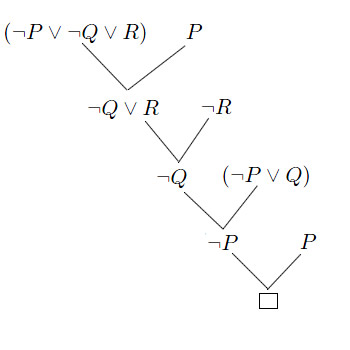
\includegraphics[height=175pt,width=175pt]{4b.jpg}

5)
	\begin{enumerate}
		\item[8.6 (a)] Some students took French in Spring 2001.
			\[ \exists s\; Student(s) \land Takes(s,\text{French,Spring 2001}) \]
		\item[8.6 (b)] Every student who takes French passes it.
			\[ \forall y\; \forall s\; (Student(s) \land Takes(s,\text{French},y)) \ra Passes(s,\text{French},y) \]
		\item[8.6 (c)] Only one student took Greek in Spring 2001.
			\begin{align*}
			 &\exists s\;  Student(s)  \land Takes(s ,\text{Greek,Spring 2001})  \land \\
			 &( \forall s'\; (Student(s') \land Takes(s',\text{Greek,Spring 2001})) \ra  =(s,s') )
			\end{align*}
		\item[8.6 (d)] The best score in Greek is always higher than the best score in French.
			\begin{align*}
			  &\forall y\;\;\;\exists bf,bg\;\;\;\forall f,g\;\;Student(g) \land Student(f) \land Student(bg) \land Student(bf) \land\\
				&Takes(f,\text{French},y) \land Takes(bf,\text{French},y) \land \\
				&( >( Score(bf,\text{French},y),Score(f,\text{French},y) )  \lor =( Score(bf,\text{French},y),Score(f,\text{French},y) ) ) \\
				&\land \\
				&Takes(g,\text{Greek},y) \land Takes(bg,\text{Greek},y) \land \\
				&( >( Score(bg,\text{Greek},y),Score(g,\text{Greek},y) )  \lor =( Score(bg,\text{Greek},y),Score(g,\text{Greek},y) ) ) \\
				&\land \\
				&>( Score(bg,\text{Greek},y), Score(bf,\text{French},y) ) \\
			\end{align*}
			Explanation: $bf$ and $bg$ represent those students who scored the highest in French and Greek respectively.
			The highest scorer for French is determined in Line 3, since by definition the highest scorer is someone whose
			score is greater or equal to all others who took French. Similarly the highest scorer is determined for Greek
			in Line 6. In Line 8, it is asserted that $bg$'s score in Greek is greater than $bf$'s score in French.
		\item[8.7 (a)] All Germans speak the same languages.
			\[ \forall x,y,l\;\;\;(German(x) \land German(y) \land Language(l) \land Speaks(x,l)) \ra Speaks(y,l)) \]
	\end{enumerate}

6.a)

\nqn
{ & & &X& & }
{ & &X& & & }
{ &X& & & & }
{Q&X&X&X&X&X}
{ &X& & & & }
{ & &X& & & }

\newpage

6.b)

\begin{table}[ht]
\begin{minipage}[ht]{0.3\linewidth}
\nqn
{ & & &X&X&X}
{ & &X&X&Q&X}
{ &X&Q&X&X&X}
{Q&X&X&X&X&X}
{ &X&X&Q&X&X}
{ &Q&X&X&X&X}
\end{minipage}
\hspace{0.5cm}
\begin{minipage}[b]{0.7\linewidth}
\csp{4}{1,2,6}{1,3,5}{2,3,5,6}{1,2,3,5,6}{1,2,3,5,6}
\aft{$V_2$ = 6}
\csp{4}{6}{1,3}{2,3,5}{1,2,5}{1,3,5}
\aft{$V_3$ = 3}
\csp{4}{6}{3}{5}{2}{1,5}
\aft{$V_4$ = 5}
\csp{4}{6}{3}{5}{2}{1}
\aft{$V_5$ = 2}
\csp{4}{6}{3}{5}{2}{}
\end{minipage}

\end{table}

No legal values left for $V_6$. Hence this is a backtrack point not a solution.

\newpage

6.c)

\begin{table}[ht]
\begin{minipage}[ht]{0.3\linewidth}
\nqn
{ &Q&X&X&X&X}
{ & &X&Q&X&X}
{ &X& &X&X&Q}
{Q&X&X&X&X&X}
{ &X&Q&X&X&X}
{ & &X&X&Q&X}
\end{minipage}
\hspace{0.5cm}
\begin{minipage}[b]{0.7\linewidth}
\csp{4}{1,2,6}{1,3,5}{2,3,5,6}{1,2,3,5,6}{1,2,3,5,6}
\aft{$V_2$ = 1}
\csp{4}{1}{3,5}{2,5,6}{2,3,5,6}{2,3,6}
\aft{$V_3$ = 5}
\csp{4}{1}{5}{2}{2,6}{3,6}
\aft{$V_4$ = 2}
\csp{4}{1}{5}{2}{6}{3,6}
\aft{$V_5$ = 6}
\csp{4}{1}{5}{2}{6}{3}
\end{minipage}
\end{table}

All the variables have values, hence this is a solution.
\newpage
6.d)

\nqn
{ & & &X&X& }
{ & &X&X& &X}
{ &X&Q&X&X&X}
{Q&X&X&X&X&X}
{ &X&X&Q&X&X}
{ &Q&X&X&X&X}

At this stage there are no values for $V_5$ and $V_6$ which don't conflict with each other.
Hence this is a backtrack point.

\end{document}